%%%%%%%%%%%%%%%%%%%%%%%%%%%%%%%%%%%%%%%%%
% 
% LaTeX Template
% Version 3.1 (25/3/14)
%
%%%%%%%%%%%%%%%%%%%%%%%%%%%%%%%%%%%%%%%%%

%----------------------------------------------------------------------------------------
%	PACKAGES AND DOCUMENT CONFIGURATIONS
%----------------------------------------------------------------------------------------

\documentclass[12pt, a4 paper]{article}

\usepackage{tikz}
%\usepackage[top=2cm, bottom=2cm, outer=0cm, inner=0cm]{geometry}
\usepackage{graphicx} % Required for the inclusion of images
\usepackage{multicol} % Required for multicolumns
\usepackage{setspace} % Required for line spacing
\setlength\parindent{0pt} % Removes all indentation from paragraphs
\setlength{\columnseprule}{0.4pt} % Adds vertical line between multicolumns
\usepackage{multirow} % Required for multirows
\usepackage{booktabs} % For prettier tables
\usepackage{xcolor}
%\usepackage{tabularx}
%\renewcommand{\rmdefault}{ptm}

%\usepackage{helvet}

\usepackage{times} % Uncomment to use the Times New Roman font

%----------------------------------------------------------------------------------------
%	DOCUMENT INFORMATION
%----------------------------------------------------------------------------------------

\begin{document}

\tikz[remember picture,overlay] \node[inner sep=0pt] at (current page.center){
\includegraphics[width=\paperwidth,height=\paperheight]{image1.jpeg}};

\clearpage

%\font\myfont=cmr12 at 35pt
%\title{\myfont  Event Name} % Write Event name here
%\author{}
%\date{\vspace{-10ex}}

%\maketitle % Insert the title, author and date
\setstretch{1.5}

%\tikz[remember picture,overlay] \node[opacity=0.8,inner sep=0pt] at (current page.center){
\includegraphics[width=\paperwidth,height=\paperheight]{Border48-A4--Arvin61r58.png}};
%\tikz[remember picture,overlay] \node[opacity=0.5,inner sep=0pt] at (current page.center){\includegraphics[width=\paperwidth,height=\paperheight]{color-2174049__340.png}};

\begin{center}
\Huge \bfseries \ttfamily SESSION ON ENTREPRENEURSHIP AWARENESS AND B-PLAN

COMPETITION
\end{center}

\begin{center}
\large Session for discussing Business ideas
\end{center}

\begin{center}
\begin{multicols}{2}
\begin{tabular}{l r}
Date: & 13/02/2019\\ % Date the event was held
Time: & 3:00 pm to 5:00 pm \\ % Time of event 
\end{tabular}
\columnbreak
\begin{tabular}{l r}
Venue: & TCC Seminar Hall \\ % Venue of event
%Total Attendance: & Number \\ % Number of participants
\end{tabular}
\end{multicols}


\begin{Large}
\begin{multicols}{2}
A session on “Entrepreneurship Awareness and B-Plan Competition” was organized on February 13, 2019 from 3:00 pm to 5:00 pm in TCC Seminar Hall of the college. This session was organized to guide students about various entrepreneurship skills.

\columnbreak
%\includegraphics[width=\linewidth]{placeholder.jpg}
  %\caption{A boat.}
  %\label{fig:boat1}
\end{multicols}

\begin{multicols}{2}

%\includegraphics[width=\linewidth]{placeholder.jpg}

\columnbreak
The  session  was  conducted  by

Prowisdom Growth.

\end{multicols}

\newpage 

%\tikz[remember picture,overlay] \node[opacity=0.8,inner sep=0pt] at (current page.center){
\includegraphics[width=\paperwidth,height=\paperheight]{5TRrp44jc.png}};
%\tikz[remember picture,overlay] \node[opacity=0.8,inner sep=0pt] at (current page.center){\includegraphics[width=\paperwidth,height=\paperheight]{md_5b0912b7c0870.png}};

\begin{multicols}{2}
The students were made to express their business ideas and to present 9 components of business model canvas. The students had to tell that their idea was solving which problem, who would be their target customers, what would their initial funding , revenue streams and value proposition.

\columnbreak
%\includegraphics[width=\linewidth]{placeholder.jpg}
  
\end{multicols}

\begin{multicols}{2}
%\includegraphics[width=\linewidth]{placeholder.jpg}

\columnbreak
After the participant presented his idea, the audience present there was allowed to question, to give suggestions or recommendations to make changes in the idea. This led to a healthy discussion in which audience was keenly

  
\end{multicols} 

\begin{multicols}{2}
involved. Also the founder of Prowisdom Growth cross questioned the participant and shared his views about the idea and also shared the ways to effectively implement the idea.


\columnbreak
%\includegraphics[width=\linewidth]{placeholder.jpg}
  
\end{multicols} 

\begin{multicols}{2}
%\includegraphics[width=\linewidth]{placeholder.jpg}

\columnbreak
Overall session was quite beneficial for all the students and definitely for future entrepreneurs.
   
\end{multicols} 

\end{Large} 
\end{center}

\newpage 

%\tikz[remember picture,overlay] \node[opacity=0.8, inner sep=0pt] at (current page.center){
\includegraphics[width=\paperwidth,height=\paperheight]{5TRrp44jc.png}};
%\tikz[remember picture,overlay] \node[opacity=0.8,inner sep=0pt] at (current page.center){\includegraphics[width=\paperwidth,height=\paperheight]{md_5b0912b7c0870.png}};

\begin{center}
\Huge Pictures Section
\end{center}

\newpage 

\tikz[remember picture,overlay] \node[opacity=0.8,inner sep=0pt] at (current page.center){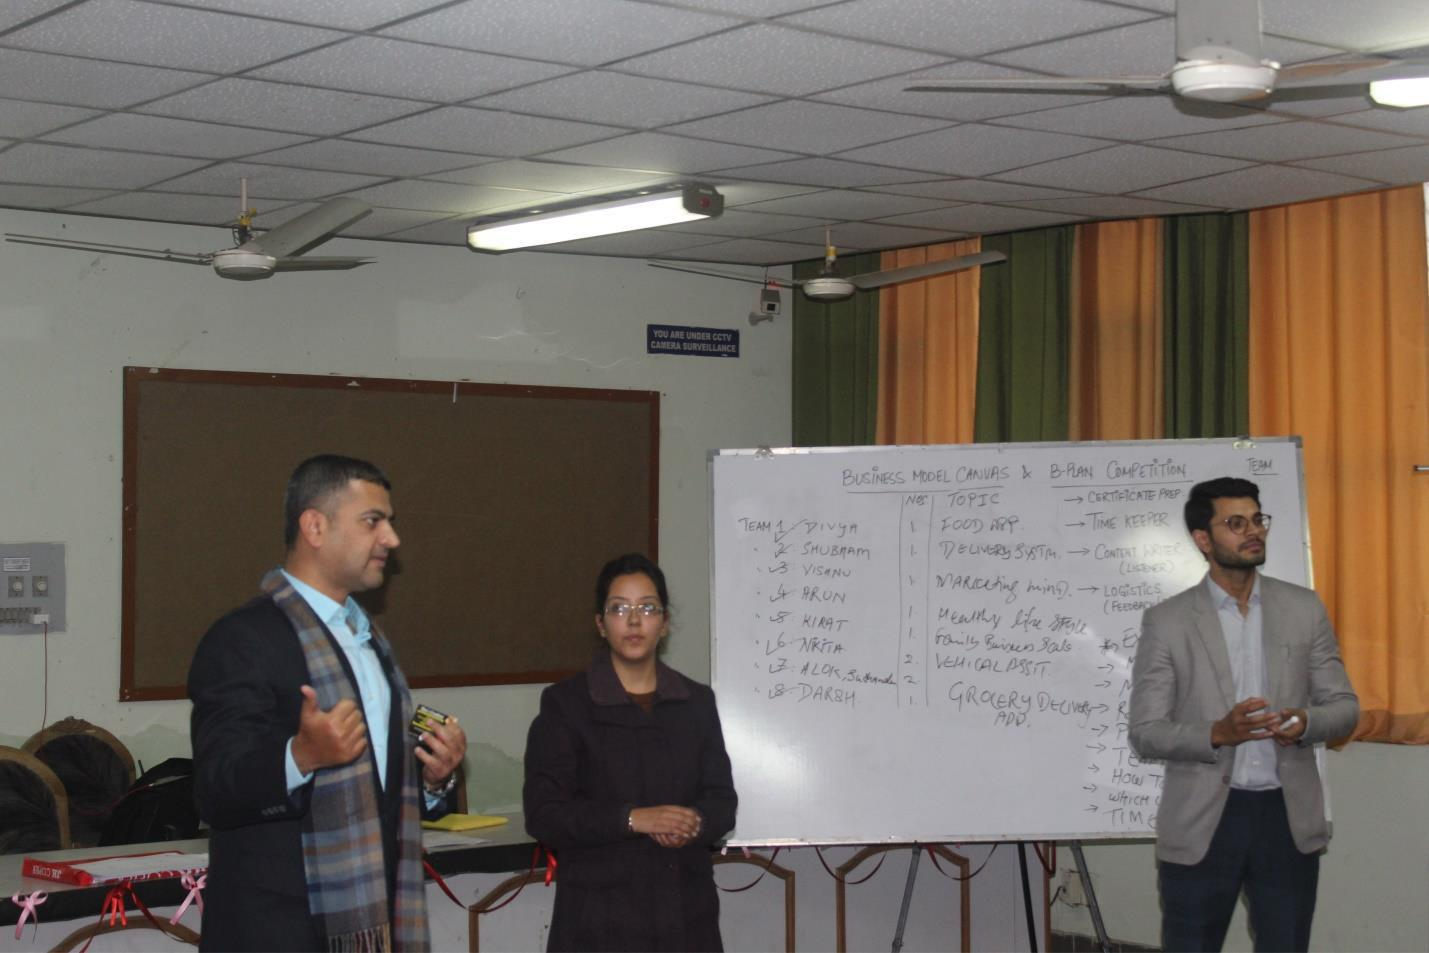
\includegraphics[width=\paperwidth,height=\paperheight]{image2.jpeg}};

\newpage

\tikz[remember picture,overlay] \node[opacity=0.8,inner sep=0pt] at (current page.center){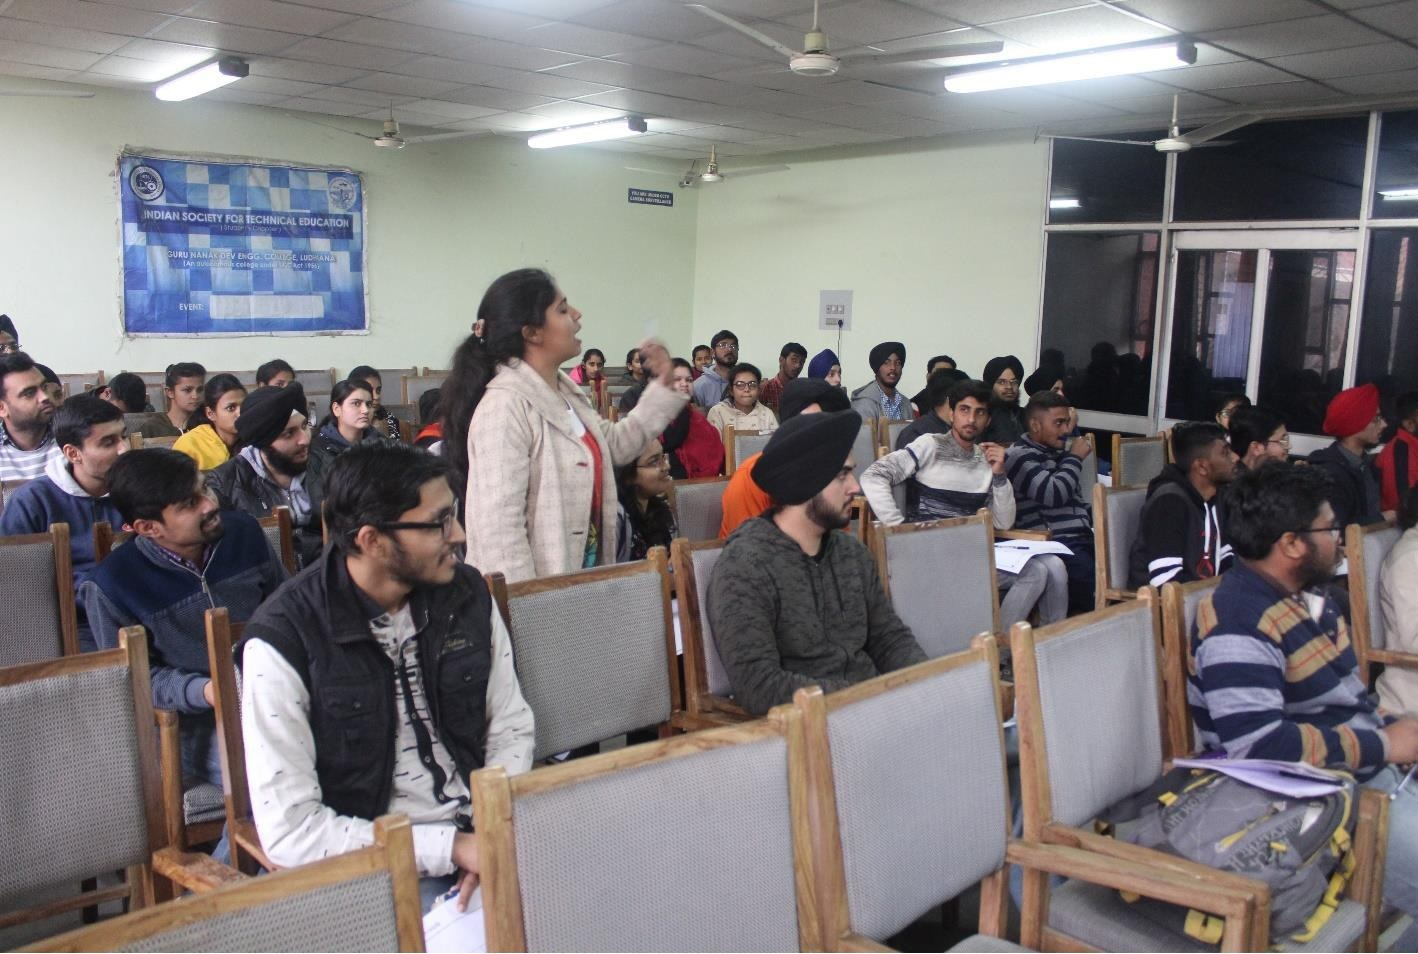
\includegraphics[width=\paperwidth,height=\paperheight]{image3.jpg}};

\newpage

\tikz[remember picture,overlay] \node[opacity=0.8,inner sep=0pt] at (current page.center){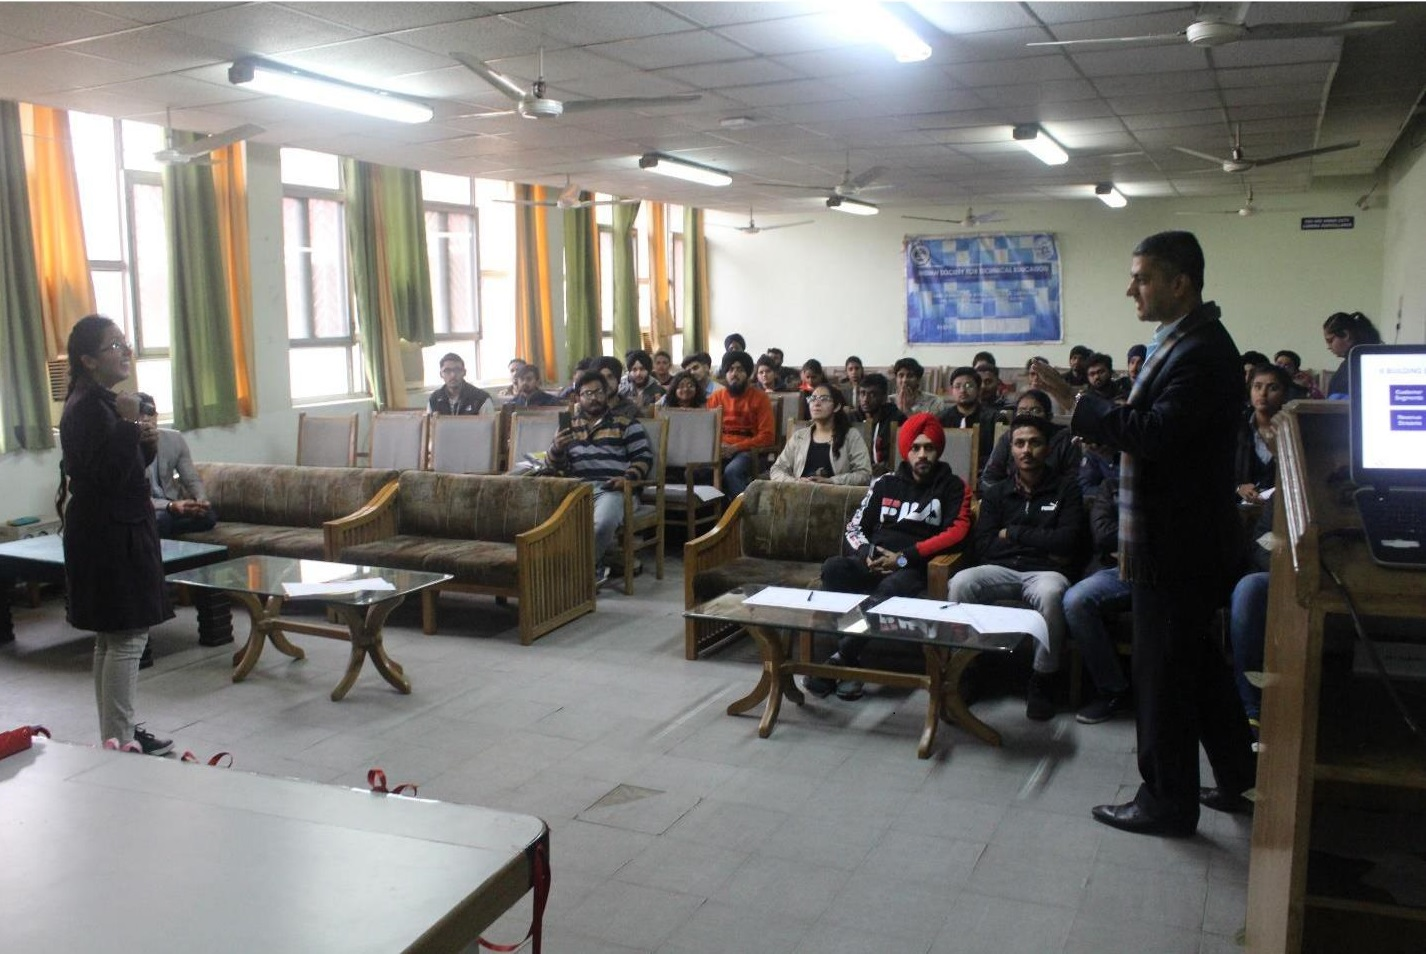
\includegraphics[width=\paperwidth,height=\paperheight]{image4.jpg}};

\newpage

\tikz[remember picture,overlay] \node[opacity=0.8,inner sep=0pt] at (current page.center){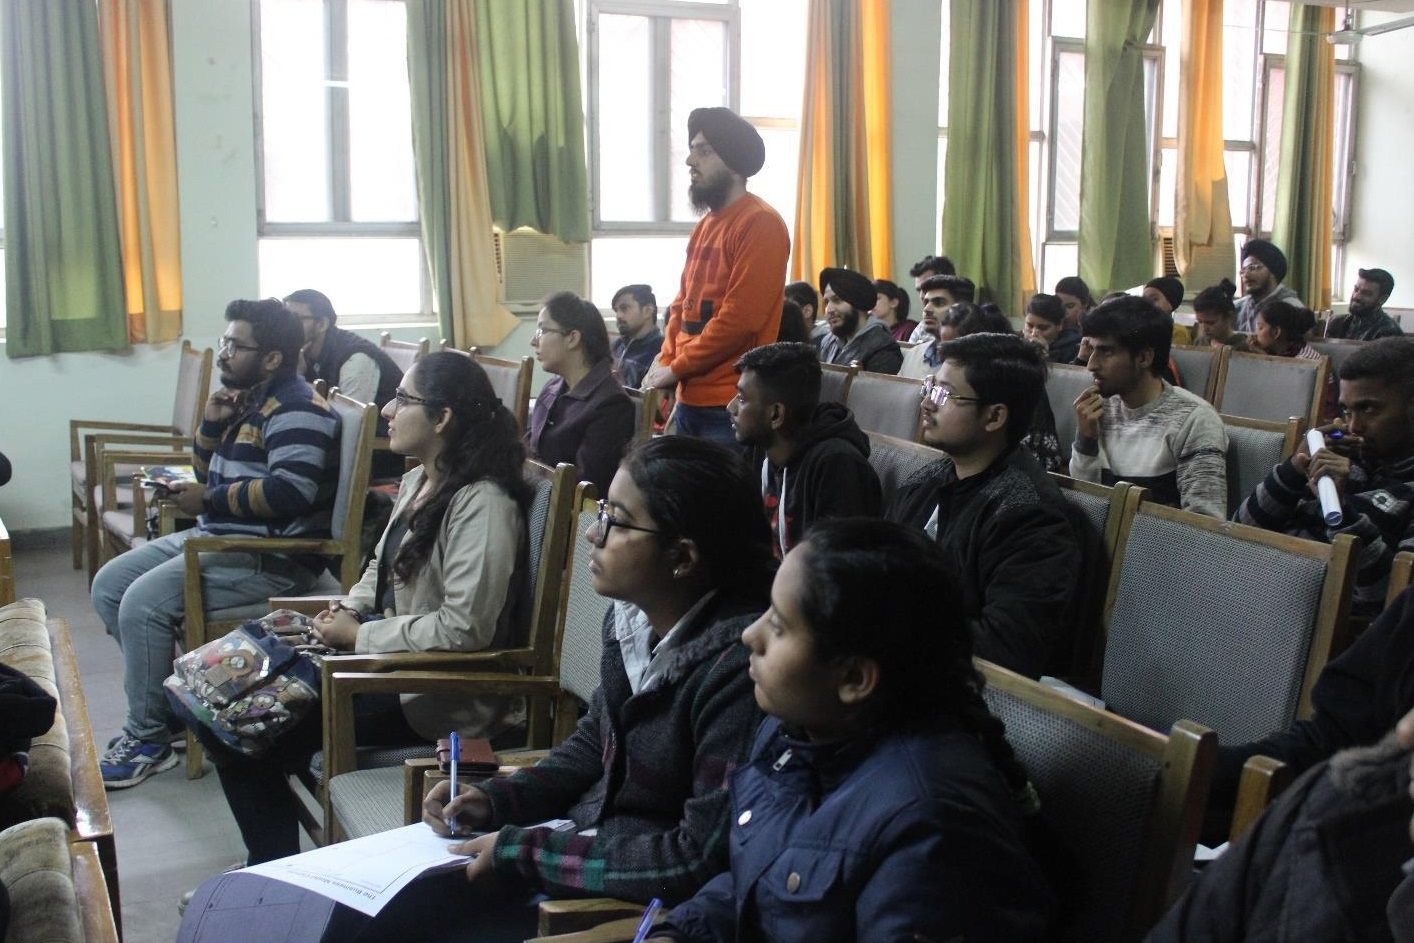
\includegraphics[width=\paperwidth,height=\paperheight]{image5.jpg}};

\newpage

\tikz[remember picture,overlay] \node[opacity=0.8,inner sep=0pt] at (current page.center){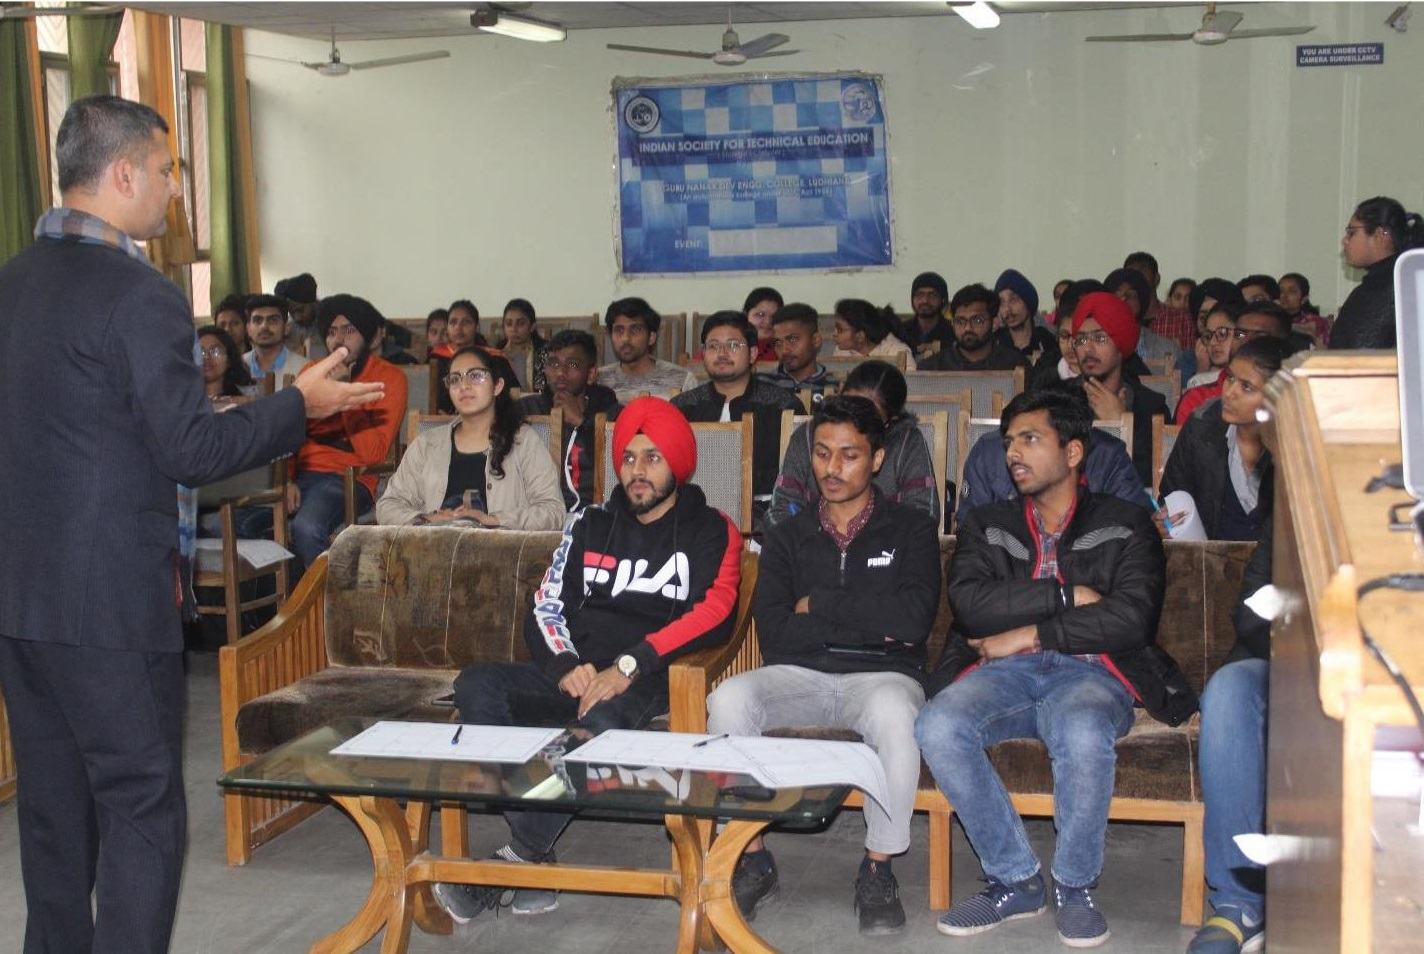
\includegraphics[width=\paperwidth,height=\paperheight]{image6.jpg}};

\newpage

\tikz[remember picture,overlay] \node[opacity=0.8,inner sep=0pt] at (current page.center){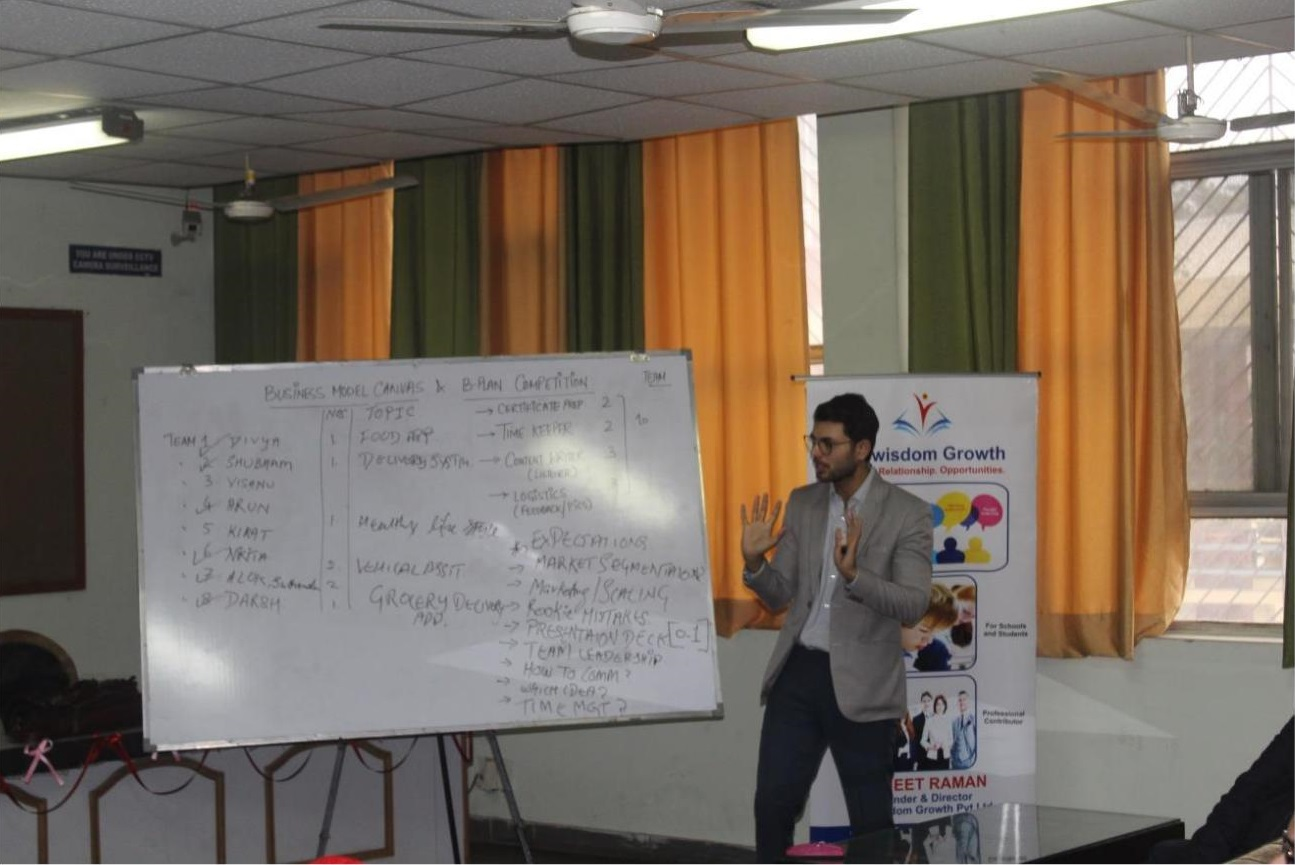
\includegraphics[width=\paperwidth,height=\paperheight]{image7.jpg}};

\newpage

\tikz[remember picture,overlay] \node[opacity=0.8,inner sep=0pt] at (current page.center){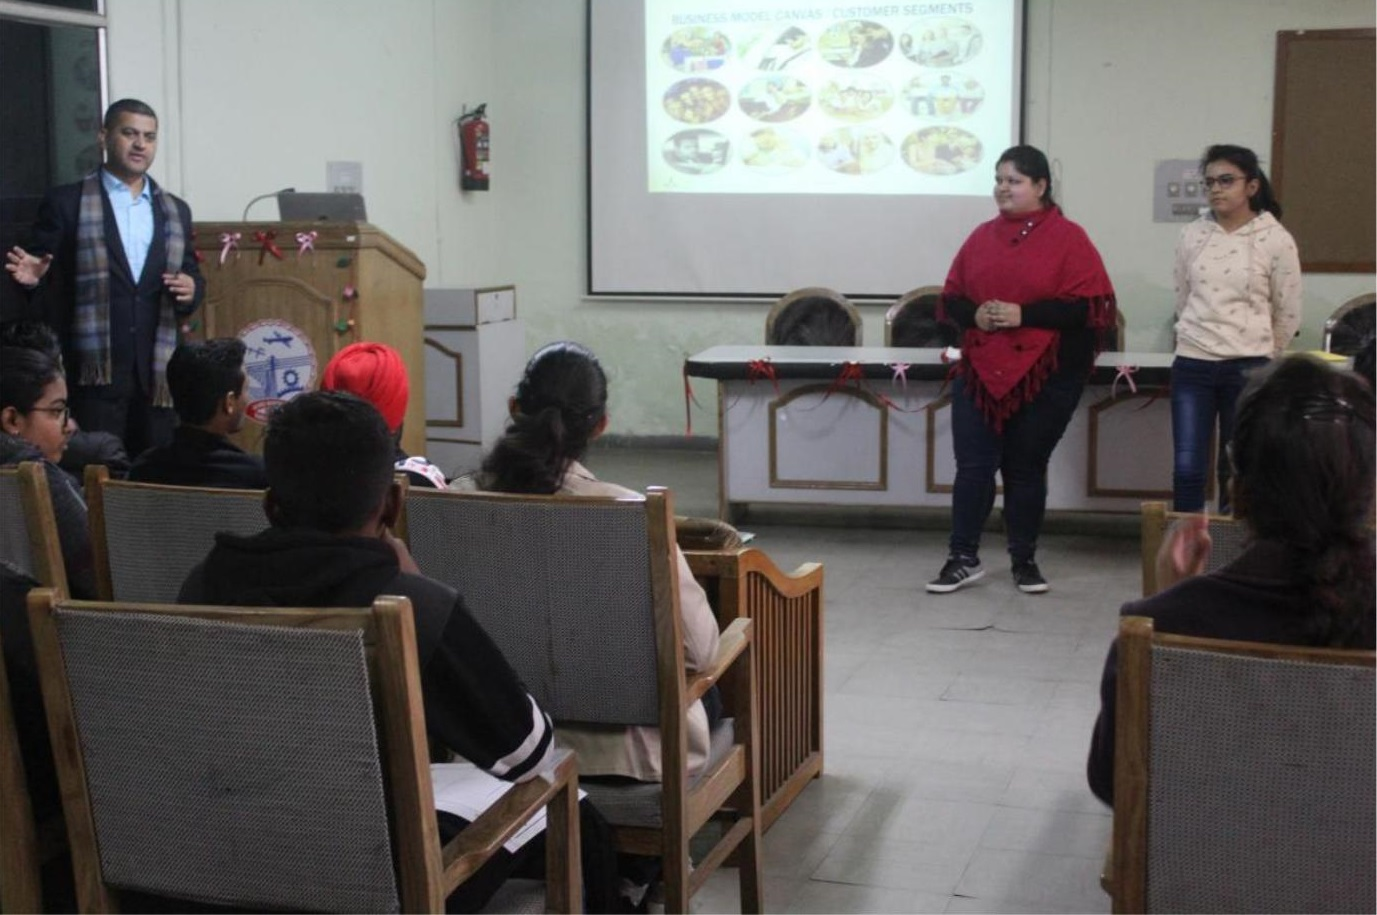
\includegraphics[width=\paperwidth,height=\paperheight]{image8.jpg}};

\newpage

\tikz[remember picture,overlay] \node[opacity=0.8,inner sep=0pt] at (current page.center){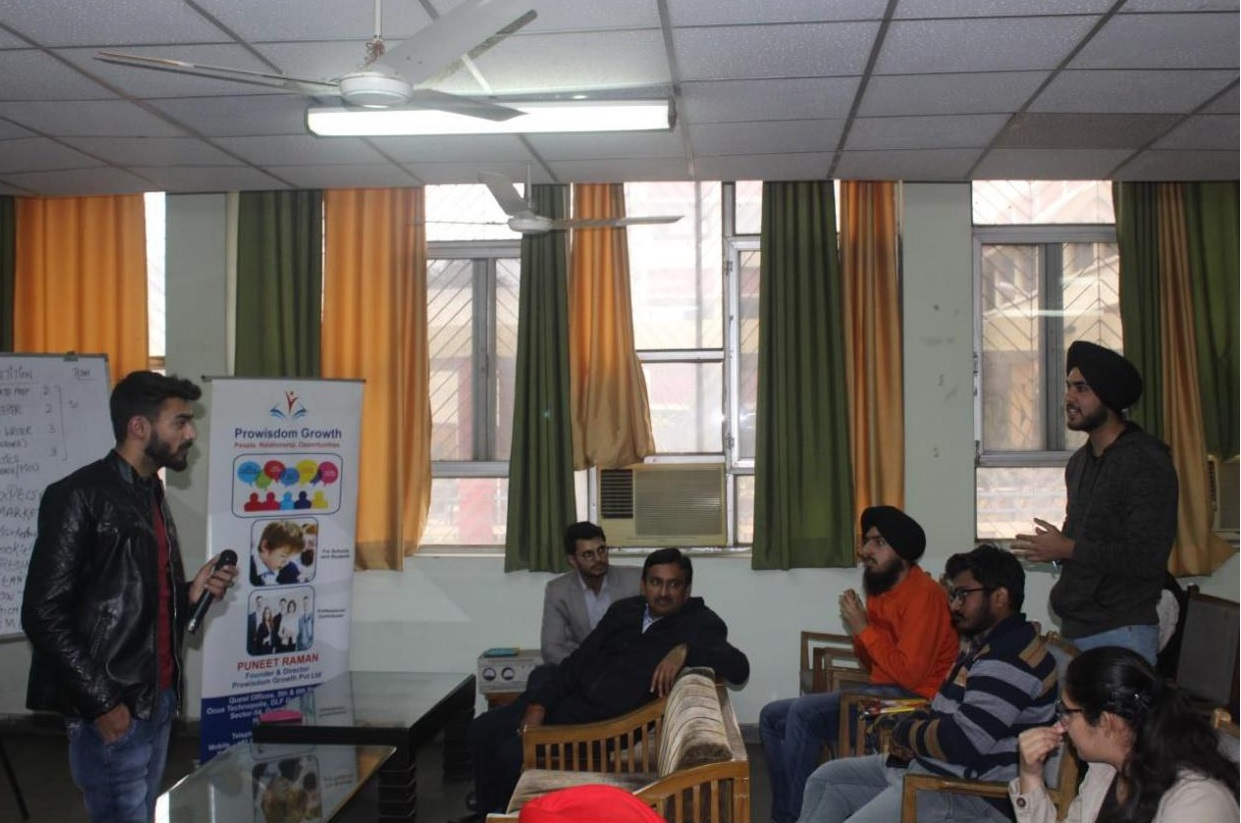
\includegraphics[width=\paperwidth,height=\paperheight]{image9.jpg}};

\newpage
\begin{center}
\huge Organisers list
\end{center}

\begin{table}[h!]
  \begin{center}
    \begin{tabular}{|c|c|c|c|c|c|} 
    \toprule % <-- Toprule here
      \textbf{S.No.} & \textbf{Name} & \textbf{Branch} & \textbf{Roll No.} \\
      \midrule % <-- Midrule here
      1 & ADITYA KHURANA & ECE & 1805372 \\
      2 & ARSHIYA GUPTA & ECE & 1805378 \\
      3 & SANCHIT KHERA & CSE & 1805220 \\
      4 & KARTIKA & CSE & 1805192 \\
      5 & KARANJOT KAUR & ECE & 1805411 \\
      6 & AMAN CHAUHAN & CSE & 1805158 \\
      7 & MANPREET & CSE & 1706471 \\
      8 & MANSIMAR SINGH & IT & 1805527 \\
      \bottomrule % <-- Bottomrule here
    \end{tabular}
  \end{center}
\end{table}

\newpage

\tikz[remember picture,overlay] \node[opacity=0.8,inner sep=0pt] at (current page.center){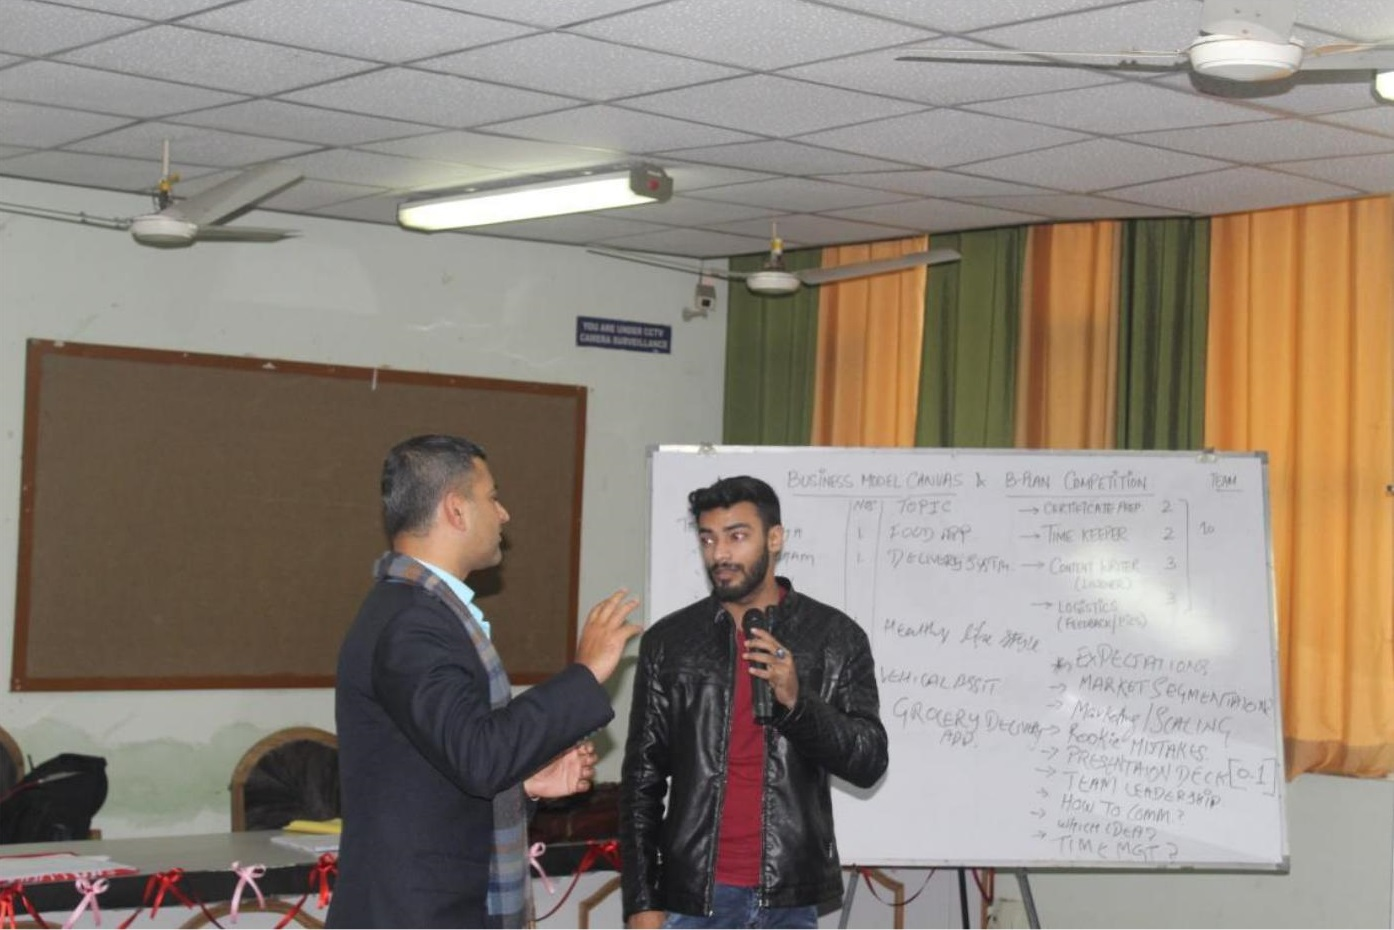
\includegraphics[width=\paperwidth,height=\paperheight]{image10.jpg}};


\end{document}